\appendix
\section{Supplementary Material}

\begin{frame}{\acs{approachname}}
    \begin{description}
    \item[\acs{approachname}] \acl{approachname}
    \end{description}

    Our contributions:
    \begin{itemize}
        \item Open-source\footnote{\url{https://github.com/KlaraGtknst/text_topic} (29.01.2025) \&\\ \url{https://github.com/KlaraGtknst/clj_exploration_leaks} (29.01.2025)}
        \item Minimal training requirements
        \item Non-textual data
        \item Information aggregation across directories      
    \end{itemize}
\end{frame}

\begin{frame}{Content of \texttt{Military} directory}
    \begin{figure}
        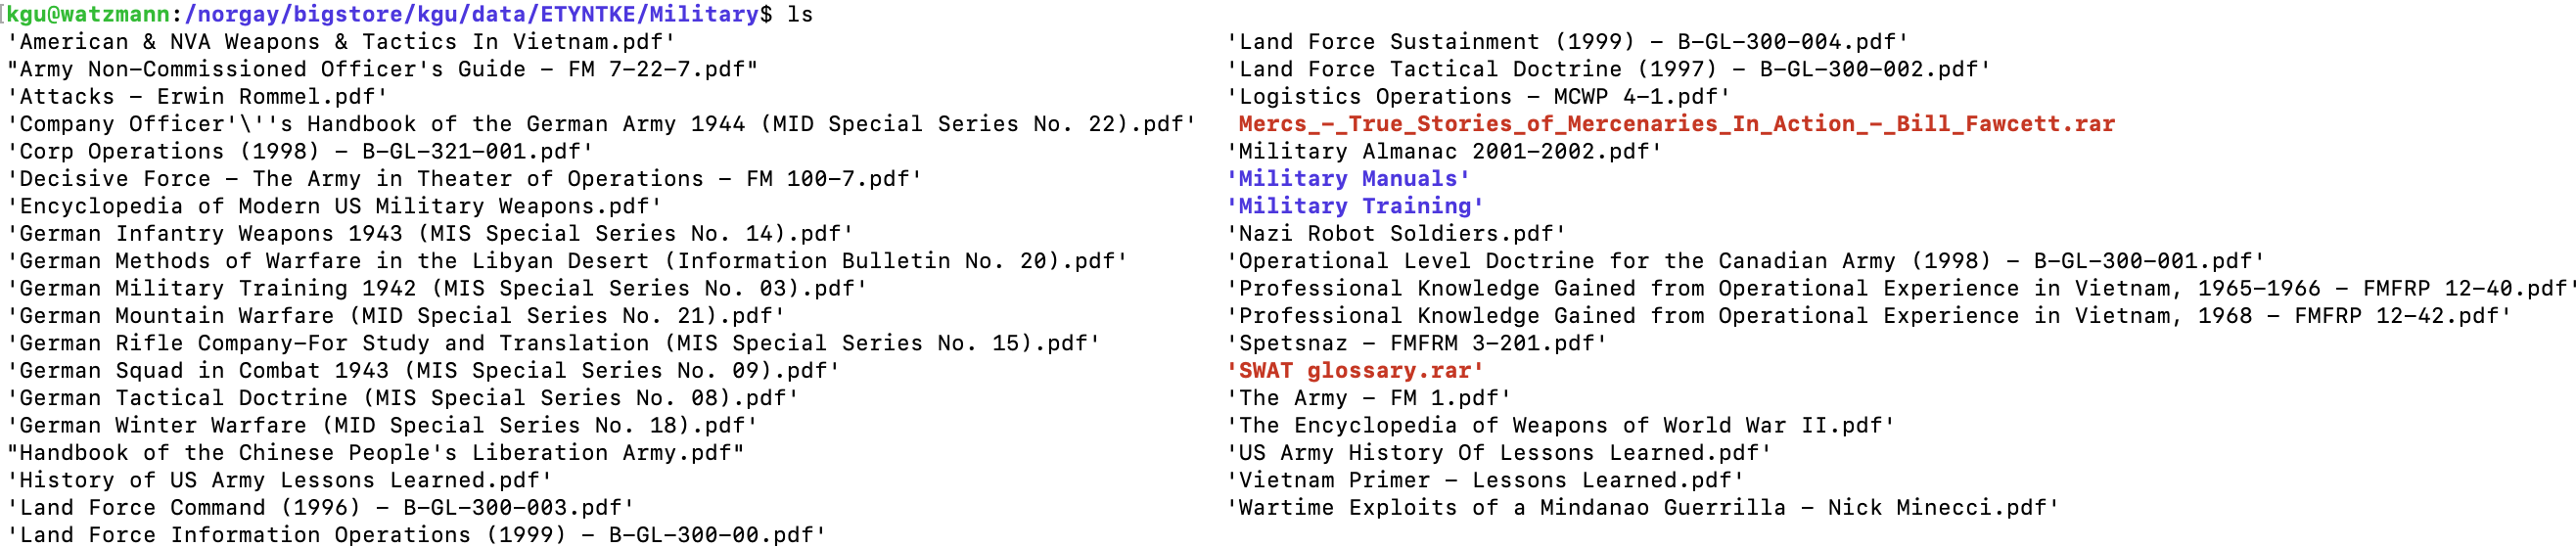
\includegraphics[width=\textwidth]{images/data_screenshots/military.png}
        \caption{Screenshot of content of \texttt{Military} directory.}
        \label{fig:military_dir_content}
    \end{figure}
\end{frame}

\begin{frame}{Content of \texttt{Business} directory}
    \only<1> {
        \begin{figure}
            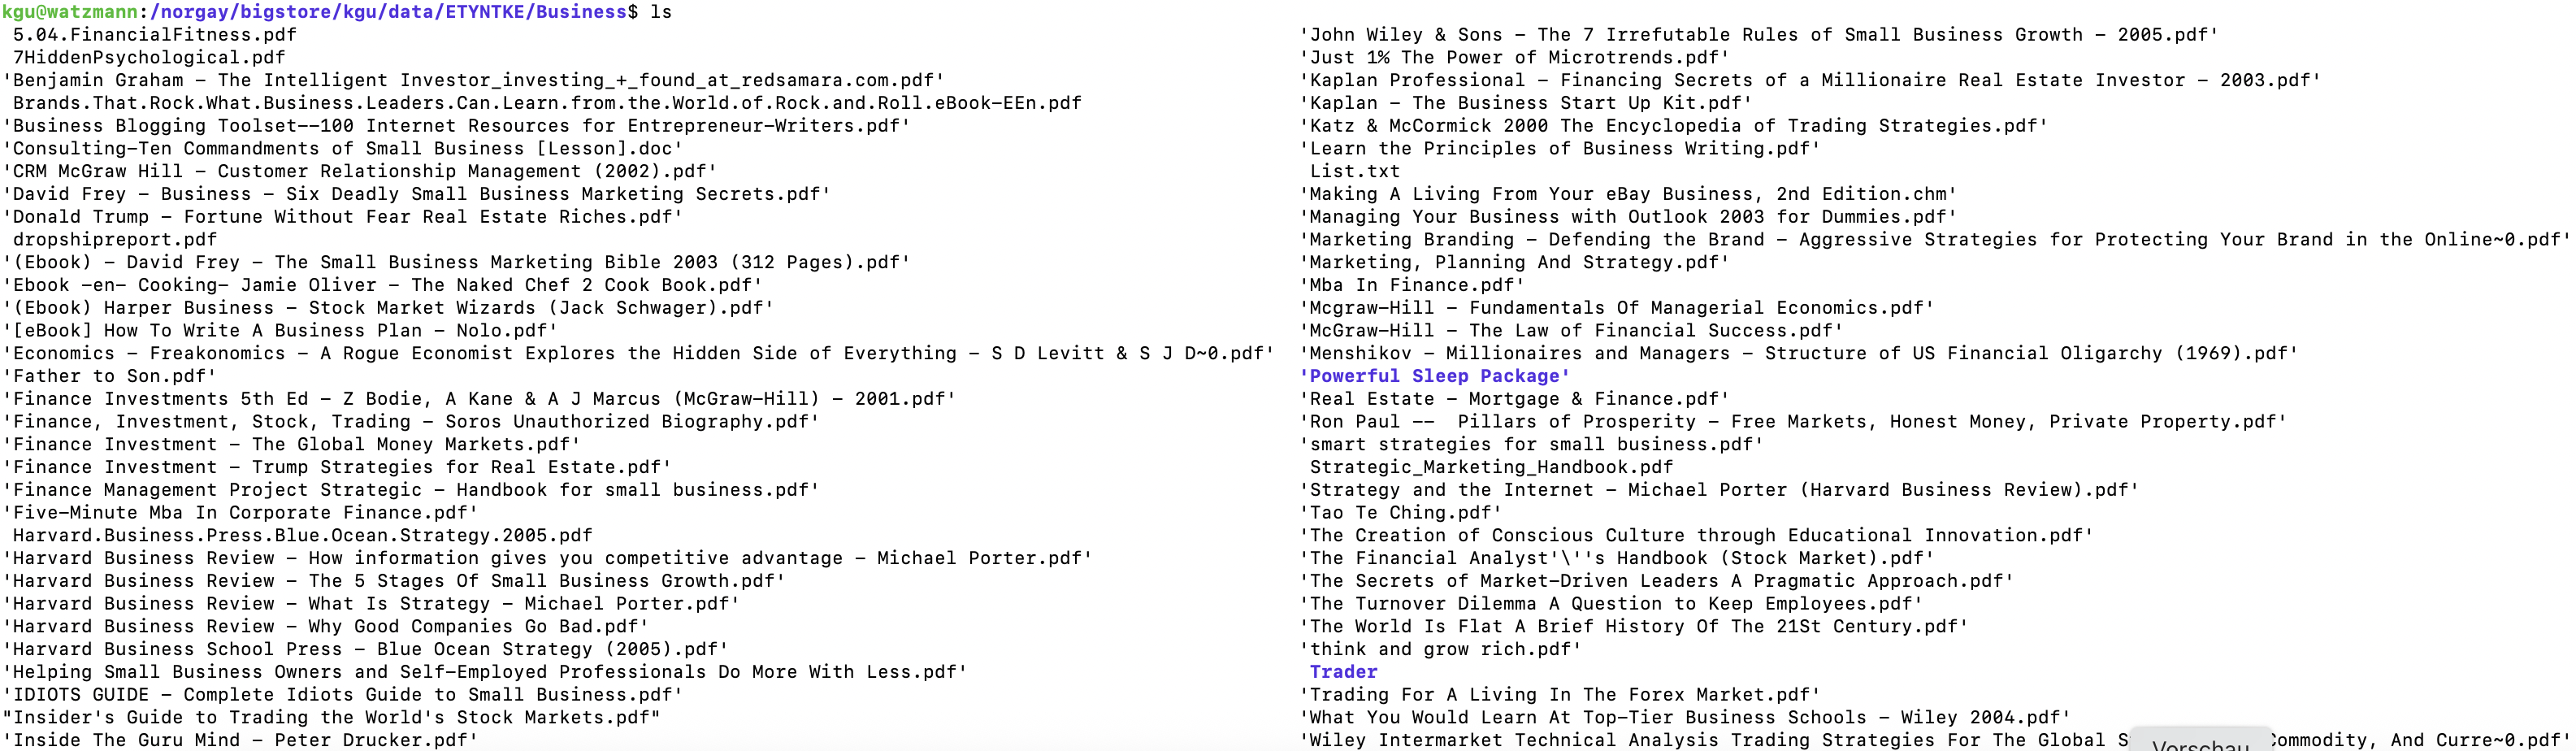
\includegraphics[width=\textwidth]{images/data_screenshots/business.png}
            \caption{Screenshot of content of \texttt{Business} directory.}
            \label{fig:business_dir_content}
        \end{figure}
    }
    \only<2> {
        \begin{figure}
            \includesvg[width=0.9\textwidth]{images/data_screenshots/wordcloud_Business.svg}
            \caption{Wordcloud\footnote{\url{https://github.com/amueller/word_cloud} (01.02.2025)} of content of \texttt{Business} directory.}
            \label{fig:business_dir_content_wordcloud}
        \end{figure}
    }
\end{frame}

\begin{frame}{Text Processing}
    \includesvg[width=\linewidth]{images/text_related_workflow}
      \vfill
    \begin{beamercolorbox}[center, wd=\linewidth, sep=1ex, rounded=true, shadow=true]{block body}
        {\small Appendix details: } 
        \hyperlink{supp:img_cap}{\beamergotobutton{Image Captioner}}
        \hspace{1em}
        \hyperlink{supp:sbert}{\beamergotobutton{\acs{sbert}}}
    \end{beamercolorbox}
\end{frame}

\begin{frame}{Image Captioner~\parencite{git_2022}}
    \label{supp:img_cap}
    \begin{figure}
        \includesvg[width=\linewidth]{images/git_image_captioner}
        \caption{\ac{git}\footnote{\url{https://huggingface.co/microsoft/git-base} (29.01.2025)}}
    \end{figure}
\end{frame}

\begin{frame}{\ac{sbert}~\parencite{sbert_2019}}
    \label{supp:sbert}
    \includesvg[width=\linewidth]{images/SentenceBERT}
\end{frame}

\begin{frame}{\ac{use}~\parencite{use_2019}}
    \label{supp:use}
    \includesvg[width=\linewidth]{images/USE}
\end{frame}